%**********************************************************************%
%* Physics for Poets Learning Notes
%* 4th edition
%* Author: Robert March
%* Chapter: 9
%* Notes: camilo tejeiro
%**********************************************************************%

% article type 12 pt font.
\documentclass[12pt, letterpaper]{article}

%----------------------- External Packages ----------------------------%
% package to insert images to our doc.
\usepackage{graphicx}

%------------------ Dimensions and Page Layout--------------------------%

%----------------------- LaTeX Environments ---------------------------%

%------------------------- LaTeX Commands -----------------------------%

%------------------------- Document Content ---------------------------%
% make title built in command values
\title{Special Relativity, A Few Thought Experiments}
\author{Learning Notes, Physics for Poets}
\date{}

\begin{document}

    \maketitle

    \section{The Postulate of Relativity}
    The central postulate of relativity is deceptively simple:
    
    \medskip\textit{The velocity of light is the same for all observers, 
    in all directions, regardless of either the observer or the light source}.
    
    \medskip
    This postulate seems innocent enough, but placing 
    an upper limit to the speed of light results in some apparent 
    counter-intuitive observations, mostly because throughout our 
    lifetime we are mostly exposed to a classical world where speeds 
    stay well below the speed of light and relativistic effects are small 
    and unnoticeable.
    
    In this little post, We shall try to explore two important by-products of 
    the postulate of relativity, mainly:
    \begin{itemize}
        \item[1. ] Time slows down for a moving object as seen from the ground.
        \item[2. ] Objects contract along their line of motion as seen from the 
        ground.
    \end{itemize}

    To start, we shall assume that the observer on the ground is ``at rest'' 
    to make our thought experiments a bit more familiar, though of course 
    the moving observer could claim he is the one ``at rest'' and he is free 
    to do so.
    
    \subsection*{Time Slows Down for a Moving Object}
    The famous train thought experiment will allow us to see how this effect 
    comes about.
    
    Let's imagine that we have the first observer inside the moving train 
    and the second observer in the ground (us) looking at the train going by.
    Now lets say that we are going to measure time by using light as our 
    measurement instrument. Because we know the speed of light is constant 
    and we can measure the distance traveled, we can calculate the time (t) 
    easily, by dividing the distance (d) by the speed of light (c) $t=d/c$. 
    
    \subsubsection*{The Observer in the Train}
    So here is how it goes, the man in the moving train is going to use his 
    flash light to time the beam of light as it goes directly from one wall 
    of the train to the other wall and back, the beam of light traveling 
    in a direction perpendicular to the train moving path (i.e. train moving 
    horizontally and light moving vertically). Then, he is going to 
    compare his measured time with the results he gets by dividing twice 
    the vertical length of the train (to account for the light return path) 
    over the speed of light $t=2l/c$.
    When he gets back to us, he is satisfied with his experiment: his 
    measured time agrees with his calculated time.       

    \begin{figure}[h!]
        \caption{The following is an illustration of what the person inside 
        the train sees (From Wikipedia):}
        \centering
        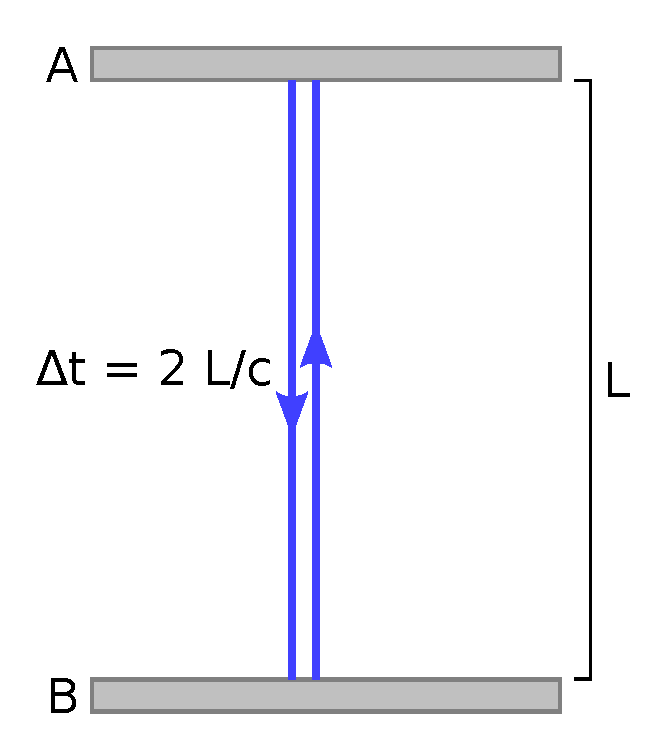
\includegraphics[scale=0.49]{time_dilation_inside_train.pdf}
    \end{figure}    
    
    \subsubsection*{The Observer in the Ground (us)}
    What we measured in the ground was completely different, 
    we got a larger measurement for the time elapsed. 
    We saw the light beam follow a diagonal path: the light beam started with a 
    vertical path but the train moved forward while the light beam was 
    traveling, so the light took longer to reach the opposite wall and come 
    back and that is exactly what we measured with our clock, so our experiment 
    agrees with our observation. 
    
    So we claim that as seen from our perspective the clock of the moving 
    observer was running slow. 
    After all the speed of light is finite and the train was traveling 
    at close to the speed of light i.e. we must consider relativistic 
    effects. And this makes perfect sense, as the train did indeed move 
    forward while the light was traveling.
    
    \begin{figure}[h!]
        \caption{The following is an illustration of what we saw looking 
        at the moving train from the ground (From Wikipedia):}
        \centering
        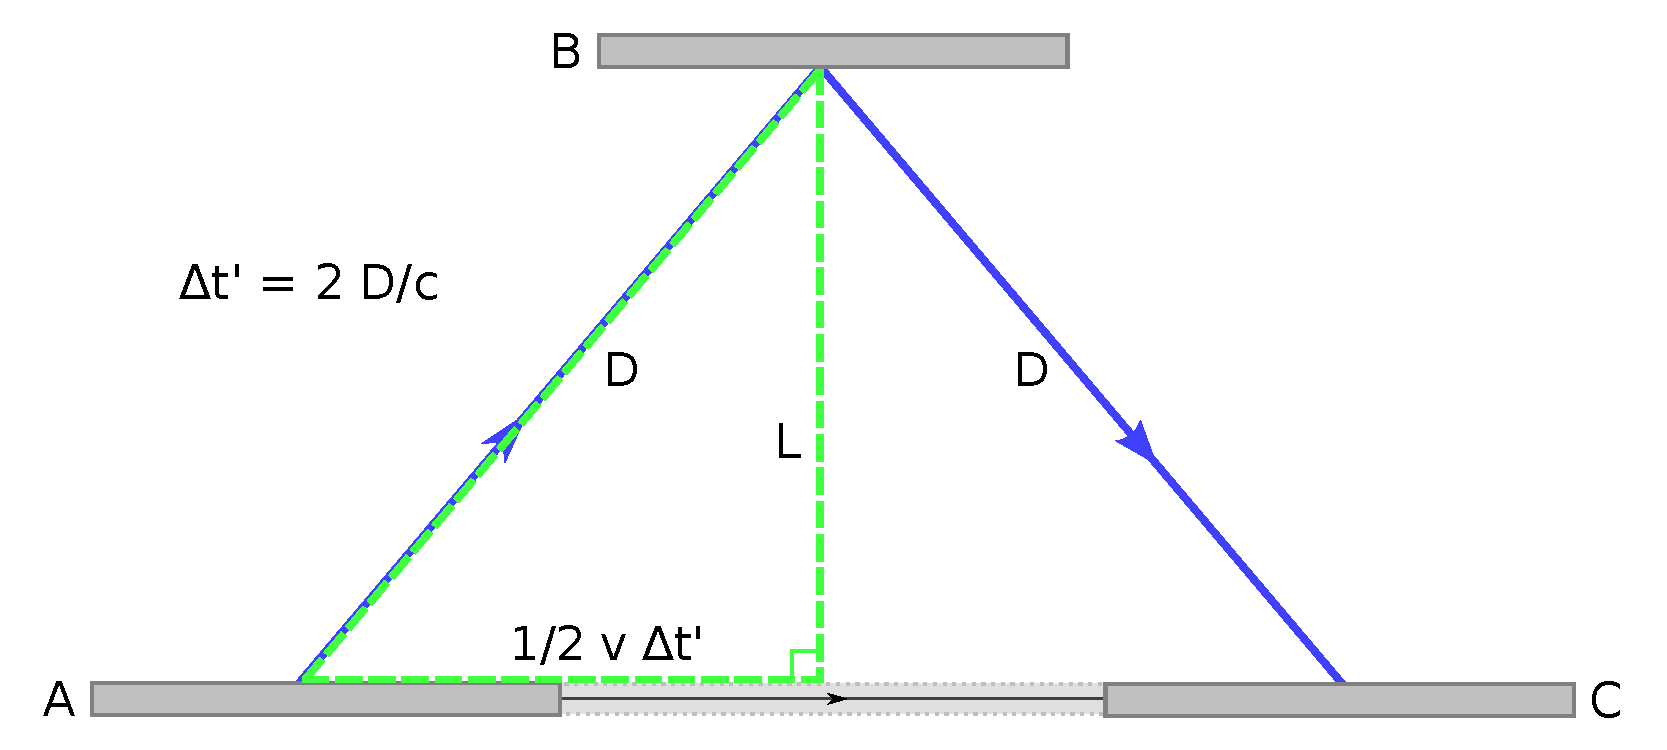
\includegraphics[scale=0.49]{time_dilation_ground.pdf}
    \end{figure}
    
    \medskip
    The truth is, both observers know what they saw but they cannot comment on 
    what the other observer saw for they where not there. Both observers are 
    correct in ``their own observations'' in ``their own frames'' and we must 
    live with that if we plan to live in a 3 dimensional world.          
    
    All we know for certain is that ``as seen from the ground'' time appears to     
    slow down for moving objects. In fact this has been proven many times 
    and sometimes we have used this knowledge to our advantage. 
    Scientists often accelerate short-lived isotopes to large speeds to be 
    able to slow their clock down enough to be able to analyze their properties 
    before they decay to lighter elements.        
    
    \subsection*{Objects Contract Along their Line of Motion}
    For this little thought experiment we can also use our beloved moving train, 
    but in this case we will be measuring the horizontal length of the train.
    
    For this we will first place distance markers on the train rail-road 
    and have two people inside the train standing at opposite sides; one person 
    all the way at the rear of the train and one person all the way at the 
    front. 
    
    Now, the idea is that if both observers inside the train look out the 
    window at the same time and record the distance seen in the 
    distance markers, we can then subtract their measurements and get the 
    length of the train. Simple, right?
    
    But just make sure that they take their measurements 
    at the same time we can use the constant speed of light to 
    synchronize their measurements. We will use a flash-light placed in the 
    middle of the train, the flash-light will go ON and then as soon as both 
    operators see the light, they will look out the window and take their 
    measurements at exactly the same time. 
    
    So here is how it goes, we start the experiment and the observers in 
    the train take their measurements, things go smoothly and they are 
    happy with their results. 
    
    But we disagree, in the ground we saw something else. The train we saw is a 
    lot shorter than they claim. You see, When the light was turned ON, 
    it moved outwards at the same speed, but the train was moving, 
    so the person in the rear of the train rushed forward to meet the light, 
    therefore he saw the light first and took his measurement too early, 
    on the other hand the person in the front of the train was moving 
    away from the light, the light had to catch up with him and so he 
    took his measurement too late. Thus when you subtract their measurements 
    you end up with a length that is too long. 
    
    \medskip
    So who is right?
    Once again, we must honor the results of both observers in their own 
    reference frames. In special relativity simultaneity does not hold for 
    all observers, i.e. events that appear simultaneous in time on one 
    reference frame (e.g. inside the moving train) might not appear so when 
    seen from another frame (e.g. at rest, outside the moving train). 
    
    
    All we can say for certain is that ``as seen from the ground'' moving objects seem 
    to compress along their line of motion.
    
\end{document}

